\chapter{\centering\normalsize{ВВЕДЕНИЕ}}
\addcontentsline{toc}{section}{ВВЕДЕНИЕ} 

 Атрибуты пользователя — это явные представления личности и характеристик человека в структурированном формате. Они предоставляют собой богатое хранилище личной информации для лучшего понимания пользователей во многих приложениях. Тем не менее, качественные пользовательские атрибуты получить сложно, поскольку информация в социальных сетях, часто распределена сильно разреженно. Таким образом, использование неструктурированных источников данных для получения структурированных пользовательских атрибутов является сложным направлением исследований.

 Между тем, люди все больше полагаются на диалоговых агентов, чтобы помогать, информировать и развлекать людей, например, составлять компанию пожилым людям и обеспечивать обслуживание клиентов. Данные о разговорах между пользователями и системами информативны и многочисленны, и большинство существующих подходов в глубоком обучении создаются на основе больших данных полученных путем crowd-source'a или извлеченных разговоров. Часто, в таких подходах учитывается только текущий контекст диалога, то есть несколько предыдущих реплик, и строится ответ на основе контекста, либо дополнительно используются атрибуты самой системы для создания последующих хороших ответов. Тем не менее, вся история диалогов одного и того же человека игнорируется, что означает, что эти системы не строят знакомство с пользователями постепенно, извлекая пользовательскую информацию из разговоров.

 Цель данной работы заключается в создании современного framework'а извлечения пользовательских атрибутов в достаточно универсальном структурированном формате из диалогов, для дальнейшего использования их в различных подзадачах, например в рекомендательных системах. Ставится задача предсказания данных о пользователях, которые представляются в формате кортежа: \emph{(субъект, отношение, объект)} из данной реплики, которые в данной работает называются "триплетами". Например, в реплике "I have walked with my dog this morning." содержится кортеж \emph{(I, have pet, dog)}. Тем не менее, стоит заметить, реплики могут содержать, либо никаких кортежей, либо сразу несколько. Например, в реплике "Good morning, how are you?" нет никакой информации о пользователе, и соответственно нет кортежа. А в предложении "I took my son to school on my black Lada yesterday." есть два кортежа: \emph{(I, have children, son)} и \emph{(I, have vehicle, car)}. Важно, так же отметить, что постановка задачи предполагает что framework принимает на вход только утверждения, а не вопросы. То есть если есть пара вопроса и ответа где выясняется существование некоторого атрибута пользователя, а ответ служит подтверждением или отрицанием, то данную пару необходимо преобразовать в одно утверждение от лица пользователя. Например, "Q: What pet do you own? A: A dog." $\implies$ "I have a dog.". Пример данной задачи можно увидеть на Рисунке \ref{fig:gtky_task}.

\begin{figure}[!ht]
    \centering
    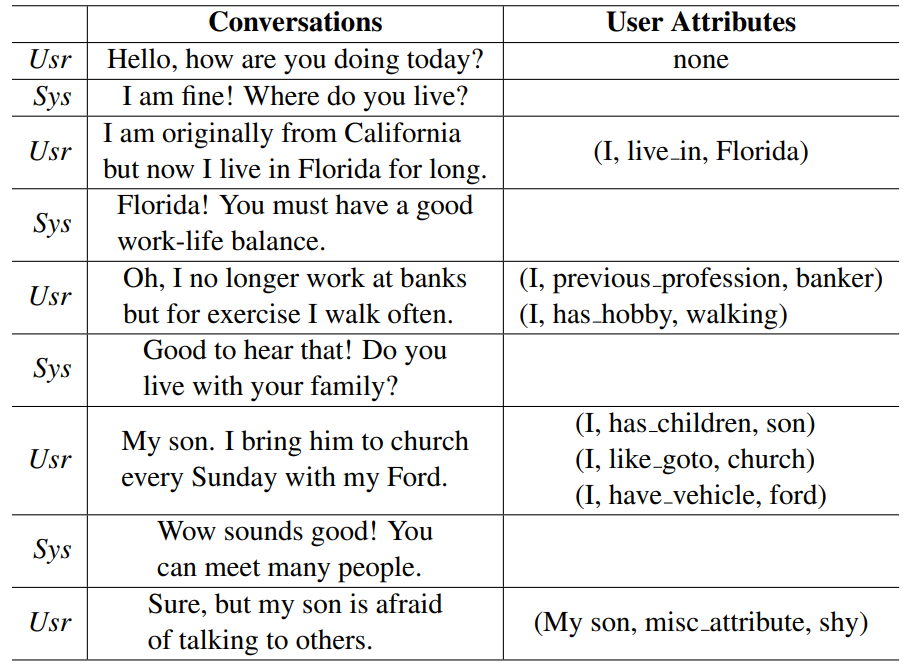
\includegraphics[width=0.8\textwidth]{images/gtky_task.png}
    \caption{Реплики и извлеченные из них кортежи. Пример взят из статьи \cite{gtky}}
    \label{fig:gtky_task}
\end{figure}

 Основную сложность в данной задаче определяет отсуствие датасета с качественной разметкой и методов обучения без учителя.
 